\documentclass[letterpaper]{article}
\usepackage[margin=1in]{geometry}
\usepackage{evan}

% Set the typeface to Times Roman
\usepackage{times}

%\usepackage{hyperref}
\usepackage{amsfonts}%
\usepackage{amssymb}%
\usepackage{amsthm}% allows theoremstyles (see below) and provides a proof environment
\usepackage{bm}
\usepackage{relsize}
\usepackage{graphicx}
\usepackage{caption}
\usepackage{epstopdf}
\usepackage{amsmath}
\usepackage{tikz}
\usetikzlibrary{trees,arrows}
\usepackage{cite}
\usetikzlibrary{decorations}
\usetikzlibrary[decorations]
\usepgflibrary{decorations.pathmorphing}
\usepgflibrary[decorations.pathmorphing]
\usetikzlibrary{decorations.pathmorphing}
\usetikzlibrary[decorations.pathmorphing]
\usepackage{booktabs}
\usepackage[authoryear]{natbib}
\usepackage{subcaption}
\usepackage{pseudocode}
%\usepackage{float}
\usepackage{verbatim} %% for commenting blocks

\bibpunct{(}{)}{,}{}{}{;} %% added this to make \citep{x} use parentheses

%% independence symbol and expectation operator %%
\newcommand\independent{\protect\mathpalette{\protect\independenT}{\perp}}
\def\independenT#1#2{\mathrel{\rlap{$#1#2$}\mkern2mu{#1#2}}}

\DeclareMathOperator*{\E}{\mathbb{E}}
\DeclareMathOperator*{\Et}{\mathbb{E}_t}
\DeclareMathOperator*{\argmax}{arg\,max}
\DeclareMathOperator{\circlearrow}{\hbox{$\circ$}\kern-1.5pt\hbox{$\rightarrow$}}
\DeclareMathOperator{\circlecircle}{\hbox{$\circ$}\kern-1.2pt\hbox{$--$}\kern-1.5pt\hbox{$\circ$}}

\newcommand\indep{\protect\mathpalette{\protect\independenT}{\perp}}
\def\independenT#1#2{\mathrel{\rlap{$#1#2$}\mkern2mu{#1#2}}}

\newtheorem{Lma}{Lemma}
\newtheorem{Thm}{Theorem}
%%%%%%%%%%%%%%%%%%%%%%%%%%%%

\title{Assignment 1}

\author{}

\date{Due: 03/08/2019 at 8pm EST}

\begin{document}

\maketitle

\section*{Problem 1}

Consider the DAG in Figure \ref{fig:prob1}.
\begin{figure}[h]
  \begin{center}
    \scalebox{0.7}{
      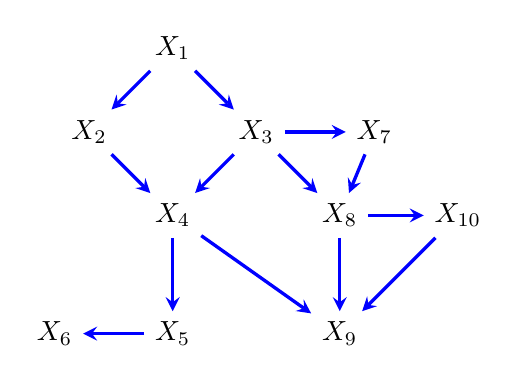
\begin{tikzpicture}[>=stealth, node distance=1.5cm]
	\tikzstyle{format} = [draw, thick, circle, minimum size=1.0mm, inner sep=0pt]
	\tikzstyle{square} = [draw, thick, minimum size=1.0mm, inner sep=3pt]
	\begin{scope}
	  \path[->, very thick]
	  node[] (x1) {$X_1$}
	  node[below left of=x1] (x2) {$X_2$}
	  node[below right of=x1] (x3) {$X_3$}		
	  node[right of=x3] (x7) {$X_7$}
	  node[below right of=x3] (x8) {$X_8$}
	  node[below left of=x3] (x4) {$X_4$}
	  node[right of=x8] (x10) {$X_{10}$}
	  node[below of=x8] (x9) {$X_9$}
	  node[below of=x4] (x5) {$X_5$}
	  node[left of=x5] (x6) {$X_6$}
	  (x1) edge[blue] (x2)
	  (x1) edge[blue] (x3)
	  (x2) edge[blue] (x4)
	  (x3) edge[blue] (x7)
	  (x3) edge[blue] (x4)
	  (x3) edge[blue] (x8)
	  (x4) edge[blue] (x5)
	  (x4) edge[blue] (x9)
	  (x5) edge[blue] (x6)
	  (x7) edge[blue] (x8)
	  (x8) edge[blue] (x9)
	  (x8) edge[blue] (x10)
	  (x10) edge[blue] (x9)
	  ;
	\end{scope}
      \end{tikzpicture}
    }
  \end{center}
  \caption{}
  \label{fig:prob1}
\end{figure}

\begin{enumerate}[a)]
  \ii List all the independencies that comprise the local Markov property for this DAG.
  \begin{answer*}
    We have the independencies
    \begin{align*}
      X_2 &\indep \left\{ X_3, X_7, X_8, X_{10} \right\}\mid X_1 \\
      X_3 &\indep X_2\mid X_1 \\
      X_4 &\indep \left\{ X_1, X_7, X_8, X_{10} \right\}\mid \left\{ X_2, X_3 \right\} \\
      X_5 &\indep \left\{ X_1, X_2, X_3, X_7, X_8, X_9, X_{10} \right\}\mid X_4 \\
      X_6 &\indep \left\{ X_1, X_2, X_3, X_4, X_7, X_8, X_9, X_{10} \right\} \mid X_5 \\
      X_7 &\indep \left\{ X_1, X_2, X_4, X_5, X_6 \right\}\mid X_3 \\
      X_8 &\indep \left\{ X_1, X_2, X_4, X_5, X_6 \right\}\mid \left\{ X_3, X_7 \right\} \\
      X_9 &\indep \left\{ X_1, X_2, X_3, X_5, X_6, X_7 \right\}\mid \left\{ X_4, X_8, X_{10} \right\} \\
      X_{10} &\indep \left\{ X_1, X_2, X_3, X_4, X_5, X_6, X_7 \right\}\mid X_8
    \end{align*}
  \end{answer*}


  \ii Is $X_2 \perp_d X_9 | X_4$? Is $X_7 \perp_d X_5 | \{X_3, X_8 \}$? Is $ \{X_2, X_4\} \perp_d X_7 | \{X_6, X_9, X_{10} \}$?
  \begin{answer*}
    $X_2\perp_d X_9\mid X_4:$ This is not true, there exists a $d$-connecting path $X_2\to X_1\to X_3\to X_8\to X_9$ where none of the intermediate vertices are colliders, yet none are $X_4.$

    $X_7\perp_d X_5\mid \left\{ X_3, X_8 \right\}:$ This is true. Every path from $X_7$ to $X_5$ must pass through either $X_3$ or $X_8,$ and neither are colliders, so there are no $d$-connecting paths.

    $\left\{ X_2, X_4 \right\}\perp_d X_7\mid \left\{ X_6, X_9, X_{10} \right\}:$ This is not true, there exists a $d$-connecting path $X_4\to X_3\to X_7$ and $X_3$ is not a collider but is not in $\left\{ X_6, X_9, X_{10} \right\}.$
  \end{answer*}

\end{enumerate}



\newpage
\section*{Problem 2}

Given a DAG $\mathcal{G}$ define: $MB(X_i,\mathcal{G}) \equiv pa(X_i) \cup ch(X_i) \cup pa(ch(X_i))$. Prove, using d-separation, that this set satisfies $X_i \indep \mathbf{X} \setminus \{MB(X_i,\mathcal{G}), X_i\} | MB(X_i, \mathcal{G})$.
\begin{proof}
  Consider $X\in \mathbf{X}\setminus \left\{ pa(X_i)\cup ch(X_i)\cup pa(ch(X_i))\cup X_i \right\},$ and consider any path $\pi$ from $X$ to $X_i.$

  If $\pi$ passes through $X_p\in pa(X_i)$ right before $X_i,$ then it cannot be $d$-connecting because $X_p$ is a non-collider yet is in $MB(X_i).$

  If $\pi$ passes through $X_c\in ch(X_i)$ right before $X_i,$ then it either went through $X_{pc}\in pa(ch(X_i))$ right before, or it did not. If it did, then $X_{pc}$ is a non-collider yet is in $MB(X_i).$ If it did not, then $X_c$ is a non-collider yet is in $MB(X_i).$

  There are no other possible paths, so since all possible $\pi$ are $d$-separated, it follows that $X_i\perp_d \mathbf{X}\setminus\left\{ MB(X_i)\cup X_i \right\}\mid MB(X_i).$ In DAGs, $d$-separation implies conditional independence, so we have the result as desired.
\end{proof}


\newpage
\section*{Problem 3}

Consider an undirected graph $\mathcal{G}$ which satisfies the local Markov property for UGs. Prove that it also satisfies the pairwise Markov property using the graphoid axioms. That is, assume that $X_i \indep \mathbf{X} \setminus cl(X_i, \mathcal{G}) | ne(X_i,\mathcal{G})$ and that $X_i \not\sim X_j$ in $\mathcal{G}$, and derive that $X_i \indep X_j | \mathbf{X} \setminus \{X_i,X_j\}$. (Hint: this is quite easy if you pick the right graphoid axiom!)
\begin{proof}
  Since $X_i\not\sim X_j,$ we know that $X_j\not\in cl(X_i)\implies X_j\in \mathbf{X}\setminus cl(X_i).$ We write $cl(X_i)=X_i\cup ne(X_i)$ and
  \begin{align*}
    \mathbf{X} \setminus cl(X_i) &= X_j\cup \left[ \mathbf{X}\setminus\left( X_j\cup X_i\cup ne(X_i) \right) \right]
  \end{align*}
  so by the graphoid axiom of weak union, we have
  \begin{align*}
    X_i\indep \mathbf{X}\setminus cl(X_i)\mid ne(X_i) &\implies X_i\indep X_j\cup \left[ \mathbf{X}\setminus\left( X_j\cup X_i\cup  ne(X_i) \right) \right] \mid ne(X_i) \\
    &\implies X_i\indep X_j\mid \mathbf{X} \setminus \left( X_j\cup X_i\cup ne(X_i) \right)\cup ne(X_i) \\
    &\implies X_i\indep X_j\mid \mathbf{X}\setminus\left\{ X_i, X_j \right\}
  \end{align*}
  as desired.
\end{proof}

\newpage
\section*{Problem 4}
\begin{enumerate}[a)]
  \ii Consider the DAG $\mathcal{G}$ in Figure \ref{fig:prob3a}. Which of the DAGs in Figure \ref{fig:prob3b} are Markov equivalent to $\mathcal{G}$? 
  \begin{answer*}
    (a) is not equivalent because $A\to B\gets C$ was unshielded in the original but is not a $v$-structure here. 

    (b) is not equivalent because $A\to B\gets C$ was unshielded in the original but is not here.

    (c) is not equivalent because $A\to E\gets C$ was unshielded in the original but is not here.

    (d) is not equivalent because $C\to E\gets A$ was unshielded in the original but is not here.

    (e) is equivalent. The original unshielded colliders $A\to E\gets C, A\to E\gets D, B\to E\gets D, A\to B\gets C$ are all preserved here

  \end{answer*}

  \ii How many DAGs are Markov equivalent to the chain $X_1 \rightarrow X_2 \rightarrow \cdots \rightarrow X_n$ (excluding itself)?
  \begin{soln}
    Any Markov equivalent DAG cannot have any colliders $X_{i}\to X_{i+1}\gets X_{i+2}.$ We can construct equivalent graphs as such: beginning from $(X_1, X_2),$ we can choose the orientation of the edge, and then continue to the right. However, as soon as an edge is assigned $\to,$ all subsequent edges must be assigned $\to,$ otherwise we will have a collider. Thus, the first $k$ edges are $\gets,$ the last $n-k-1$ edges must be $\to,$ where $k$ ranges from 1 (since we are excluding the original DAG) to $n-1,$ so there are $n-1$ equivalent DAGs
  \end{soln}

\end{enumerate}

\begin{figure}[h]
  \begin{center}
    \scalebox{0.7}{
      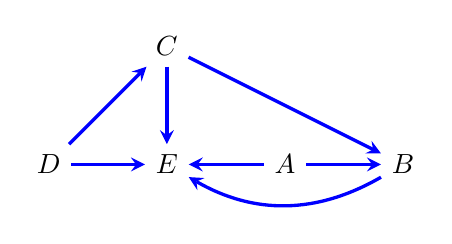
\begin{tikzpicture}[>=stealth, node distance=1.5cm]
	\tikzstyle{format} = [draw, thick, circle, minimum size=1.0mm, inner sep=0pt]
	\tikzstyle{square} = [draw, thick, minimum size=1.0mm, inner sep=3pt]
	\begin{scope}
	  \path[->, very thick]
	  node[] (C) {$C$}
	  node[below of=C] (E) {$E$}
	  node[right of=E] (A) {$A$}
	  node[left of=E] (D) {$D$}
	  node[right of=A] (B) {$B$}
	  (A) edge[blue] (B)
	  (A) edge[blue] (E) 
	  (B) edge[blue, bend left] (E)
	  (C) edge[blue] (B)
	  (D) edge[blue] (C)
	  (D) edge[blue] (E)
	  (C) edge[blue] (E)
	  ;
	\end{scope}
      \end{tikzpicture}
    }
  \end{center}
  \caption{}
  \label{fig:prob3a}
\end{figure}

\begin{figure}[h]
  \begin{center}
    \scalebox{0.7}{
      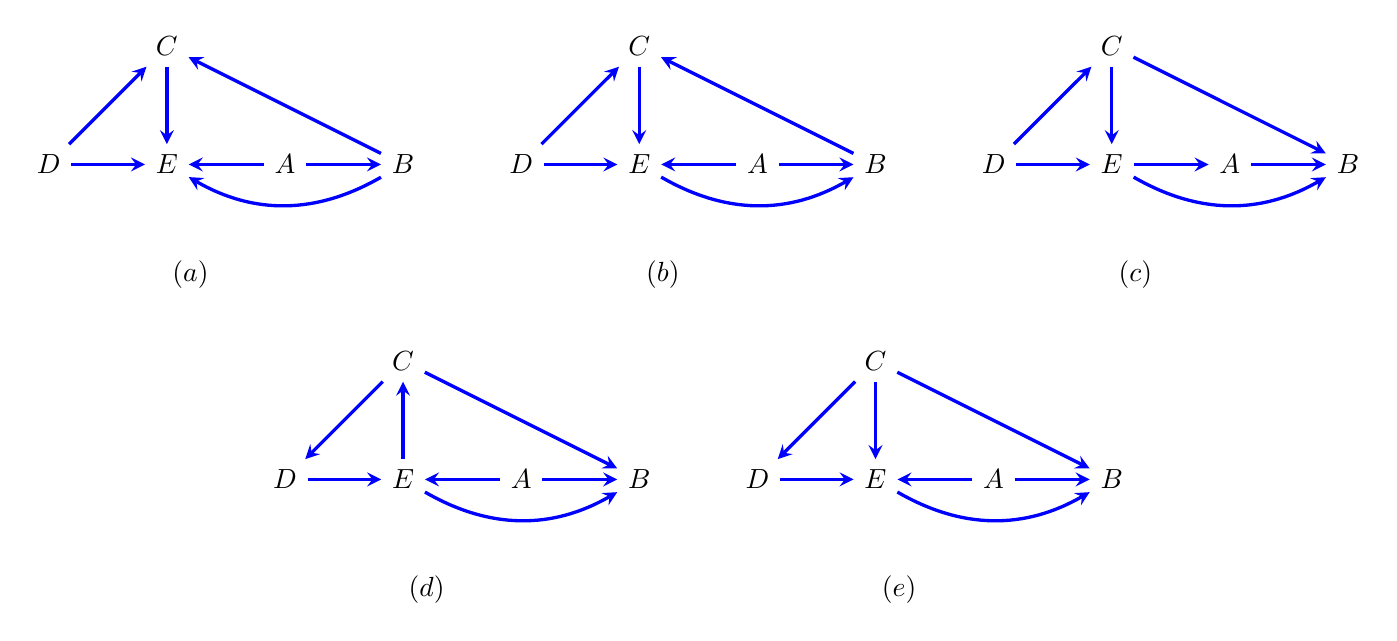
\begin{tikzpicture}[>=stealth, node distance=1.5cm]
	\tikzstyle{format} = [draw, thick, circle, minimum size=1.0mm, inner sep=0pt]
	\tikzstyle{square} = [draw, thick, minimum size=1.0mm, inner sep=3pt]
	\begin{scope}
	  \path[->, very thick]
	  node[] (C) {$C$}
	  node[below of=C] (E) {$E$}
	  node[right of=E] (A) {$A$}
	  node[left of=E] (D) {$D$}
	  node[right of=A] (B) {$B$}
	  (A) edge[blue] (B)
	  (A) edge[blue] (E) 
	  (B) edge[blue, bend left] (E)
	  (B) edge[blue] (C)
	  (D) edge[blue] (C)
	  (D) edge[blue] (E)
	  (C) edge[blue] (E)
	  node[below of=E, yshift=0.1cm, xshift=0.3cm] (l) {$(a)$}	
	  ;
	\end{scope}
	\begin{scope}[xshift=6.0cm]
	  \path[->, very thick]
	  node[] (C) {$C$}
	  node[below of=C] (E) {$E$}
	  node[right of=E] (A) {$A$}
	  node[left of=E] (D) {$D$}
	  node[right of=A] (B) {$B$}
	  (A) edge[blue] (B)
	  (A) edge[blue] (E) 
	  (E) edge[blue, bend right] (B)
	  (B) edge[blue] (C)
	  (D) edge[blue] (C)
	  (D) edge[blue] (E)
	  (C) edge[blue] (E)
	  node[below of=E, yshift=0.1cm, xshift=0.3cm] (l) {$(b)$}	
	  ;
	\end{scope}
	\begin{scope}[xshift=12.0cm]
	  \path[->, very thick]
	  node[] (C) {$C$}
	  node[below of=C] (E) {$E$}
	  node[right of=E] (A) {$A$}
	  node[left of=E] (D) {$D$}
	  node[right of=A] (B) {$B$}
	  (A) edge[blue] (B)
	  (E) edge[blue] (A) 
	  (E) edge[blue, bend right] (B)
	  (C) edge[blue] (B)
	  (D) edge[blue] (C)
	  (D) edge[blue] (E)
	  (C) edge[blue] (E)
	  node[below of=E, yshift=0.1cm, xshift=0.3cm] (l) {$(c)$}	
	  ;
	\end{scope}
	\begin{scope}[xshift=3.0cm, yshift=-4cm]
	  \path[->, very thick]
	  node[] (C) {$C$}
	  node[below of=C] (E) {$E$}
	  node[right of=E] (A) {$A$}
	  node[left of=E] (D) {$D$}
	  node[right of=A] (B) {$B$}
	  (A) edge[blue] (B)
	  (A) edge[blue] (E) 
	  (E) edge[blue, bend right] (B)
	  (C) edge[blue] (B)
	  (C) edge[blue] (D)
	  (D) edge[blue] (E)
	  (E) edge[blue] (C)
	  node[below of=E, yshift=0.1cm, xshift=0.3cm] (l) {$(d)$}	
	  ;
	\end{scope}
	\begin{scope}[xshift=9.0cm, yshift=-4cm]
	  \path[->, very thick]
	  node[] (C) {$C$}
	  node[below of=C] (E) {$E$}
	  node[right of=E] (A) {$A$}
	  node[left of=E] (D) {$D$}
	  node[right of=A] (B) {$B$}
	  (A) edge[blue] (B)
	  (A) edge[blue] (E) 
	  (E) edge[blue, bend right] (B)
	  (C) edge[blue] (B)
	  (C) edge[blue] (D)
	  (D) edge[blue] (E)
	  (C) edge[blue] (E)
	  node[below of=E, yshift=0.1cm, xshift=0.3cm] (l) {$(e)$}	
	  ;
	\end{scope}
      \end{tikzpicture}
    }
  \end{center}
  \caption{}
  \label{fig:prob3b}
\end{figure}


\newpage
\section*{Problem 5}

Consider the DAG $\mathcal{G}$ in Figure \ref{fig:prob1} and it's moralized graph $\mathcal{G}^m$.
\begin{center}
  \scalebox{0.7}{
    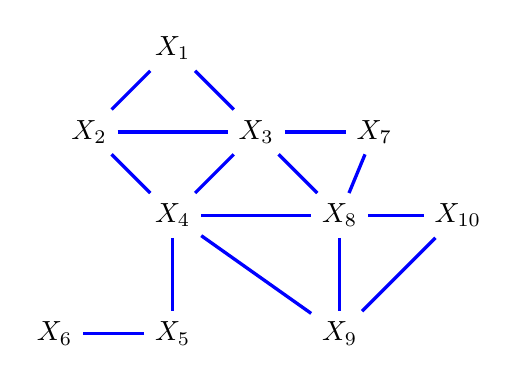
\begin{tikzpicture}[node distance=1.5cm]
      \tikzstyle{format} = [draw, thick, circle, minimum size=1.0mm, inner sep=0pt]
      \tikzstyle{square} = [draw, thick, minimum size=1.0mm, inner sep=3pt]
      \begin{scope}
	\path[-, very thick]
	node[] (x1) {$X_1$}
	node[below left of=x1] (x2) {$X_2$}
	node[below right of=x1] (x3) {$X_3$}		
	node[right of=x3] (x7) {$X_7$}
	node[below right of=x3] (x8) {$X_8$}
	node[below left of=x3] (x4) {$X_4$}
	node[right of=x8] (x10) {$X_{10}$}
	node[below of=x8] (x9) {$X_9$}
	node[below of=x4] (x5) {$X_5$}
	node[left of=x5] (x6) {$X_6$}
	(x1) edge[blue] (x2)
	(x1) edge[blue] (x3)
	(x2) edge[blue] (x4)
	(x2) edge[blue] (x3)
	(x3) edge[blue] (x7)
	(x3) edge[blue] (x4)
	(x3) edge[blue] (x8)
	(x4) edge[blue] (x5)
	(x4) edge[blue] (x8)
	(x4) edge[blue] (x9)
	(x5) edge[blue] (x6)
	(x7) edge[blue] (x8)
	(x8) edge[blue] (x9)
	(x8) edge[blue] (x10)
	(x10) edge[blue] (x9)
	;
      \end{scope}
    \end{tikzpicture}
  }
\end{center}

\begin{enumerate}[a)]

  \ii How many factor potentials appear in the factorization property for $\mathcal{G}^m$, when the factorization is by \emph{maximal} cliques?
  \begin{answer*}
    The moralized graph is shown above. Here, the maximal cliques are the 3-cliques and the pairs $(X_4, X_5)$ and $(X_5, X_6).$ Thus, there are 8 factor potentials.
  \end{answer*}

  \ii If each factor is parameterized by one parameter for each variable which appears in its scope, plus one parameter for each pair in the scope, and one for each three-way interaction (each triple in the scope), and so on... how many parameters are there in total in this representation of the joint distribution? (You can assume that the single-variable parameters appear only once for each variable, so you're not ``double counting'' when the same variable appears in multiple cliques.)
  \begin{answer*}
    There are 10 parameters for the individual variables, 15 parameters for the pairwise interactions, and 6 parameters for the three-way interactions, for a total of 31 parameters.
  \end{answer*}

  \ii How many parameters would be required to specify the joint without a graphical model, assuming binary variables?
  \begin{answer*}
    There are 10 variables, and thus $2^{10}-1=1023$ parameters required.
  \end{answer*}

  \ii How many parameters would be required to specify the joint using the DAG factorization, assuming binary variables?
  \begin{answer*}
    We have the factorization
    \begin{align*}
      p(\mathbf{x}) &= p(x_1) p(x_2\mid x_1) p(x_3\mid x_1) p(x_4\mid x_2, x_3)p(x_5\mid x_4)p(x_6\mid x_5) p(x_7\mid x_3) \\
     & \times p(x_8\mid x_3, x_7) p(x_9\mid x_4, x_8, x_{10}) p(x_{10}\mid x_8)
    \end{align*}
    In general, for a conditional probability of the form $p(x_i\mid x_{j_1}, x_{j_2}\dots x_{j_n}),$ we require $2(2^n-1)$ parameters because there are $2^{n}-1$ parameters for the conditioned variables (since the last one is determined) for each possible value of $x_i.$ Thus, the total number of parameters needed is
    \begin{align*}
      1 + 2(2-1) + 2(2-1) + 2(2-1) + 2(2-1) + 2(2-1) + 2(2-1) + 2(2^2-1) + 2(2^3-1) + 2(2-1)=  35
    \end{align*}
  \end{answer*}

  \ii How many factor potentials appear when the MRF factorization is by pairwise cliques?
  \begin{answer*}
    There are 15 pairwise cliques.
  \end{answer*}

  \ii How many parameters are there total in this latter representation of the joint distribution, with same scheme as above?
  \begin{answer*}
    There are 10 parameters for the individual variables and 15 parameters for the pairwise interactions, for a total of 25 parameters.
  \end{answer*}

\end{enumerate}
\newpage
\section*{Problem 6}

\begin{figure}[h]
  \begin{center}
    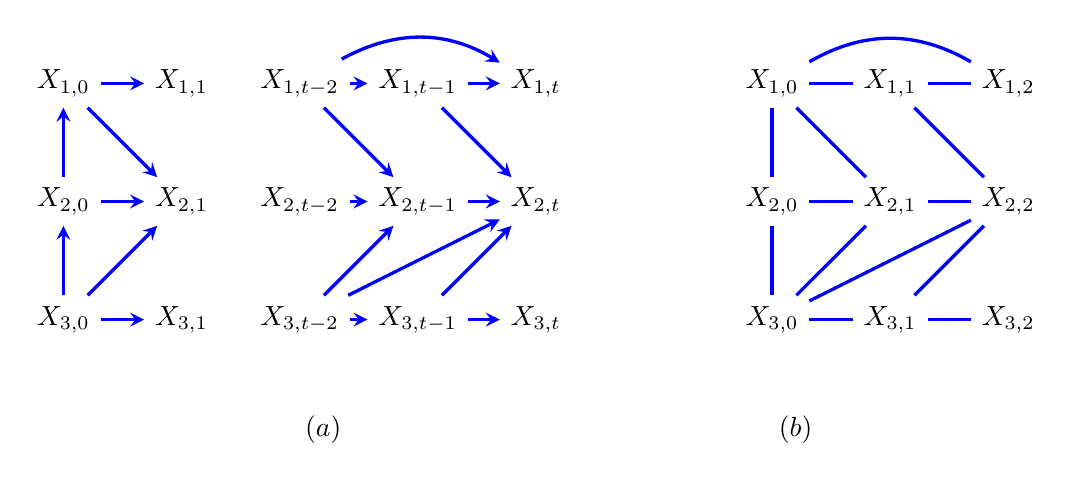
\begin{tikzpicture}[>=stealth, node distance=1.5cm]
      \tikzstyle{format} = [draw, thick, circle, minimum size=1.0mm, inner sep=0pt]
      \tikzstyle{square} = [draw, thick, minimum size=1.0mm, inner sep=3pt]
      \begin{scope}
	\path[->, very thick]
	node[] (x1) {$X_{1, 0}$}
	node[below of=x1] (x2) {$X_{2, 0}$}
	node[below of=x2] (x3) {$X_{3, 0}$}
	node[right of=x1] (x11) {$X_{1, 1}$}
	node[below of=x11] (x21) {$X_{2, 1}$}
	node[below of=x21] (x31) {$X_{3, 1}$}				
	(x3) edge[blue] (x2)
	(x2) edge[blue] (x1)
	(x1) edge[blue] (x11)
	(x2) edge[blue] (x21)
	(x3) edge[blue] (x31)
	(x1) edge[blue] (x21)
	(x3) edge[blue] (x21)
	;
      \end{scope}
      \begin{scope}[xshift=3.0cm]
	\path[->, very thick]
	node[] (x1) {$X_{1, t-2}$}
	node[below of=x1] (x2) {$X_{2, t-2}$}
	node[below of=x2] (x3) {$X_{3, t-2}$}	
	node[right of=x1] (x11) {$X_{1, t-1}$}	
	node[right of=x2] (x21) {$X_{2, t-1}$}
	node[right of=x3] (x31) {$X_{3, t-1}$}
	node[right of=x11] (x12) {$X_{1, t}$}	
	node[right of=x21] (x22) {$X_{2, t}$}
	node[right of=x31] (x32) {$X_{3, t}$}
	(x1) edge[blue] (x11)
	(x1) edge[blue] (x21)
	(x2) edge[blue] (x21)
	(x3) edge[blue] (x31)
	(x3) edge[blue] (x21)
	(x3) edge[blue] (x22)
	(x11) edge[blue] (x12)
	(x11) edge[blue] (x22)
	(x21) edge[blue] (x22)
	(x31) edge[blue] (x32)
	(x31) edge[blue] (x22)
	(x1) edge[blue, bend left] (x12)
	node[below of=x3, yshift=0.1cm, xshift=0.3cm] (l) {$(a)$}	
	;
      \end{scope}
      \begin{scope}[xshift=9.0cm]
	\path[->, very thick]
	node[] (x1) {$X_{1, 0}$}
	node[below of=x1] (x2) {$X_{2, 0}$}
	node[below of=x2] (x3) {$X_{3, 0}$}	
	node[right of=x1] (x11) {$X_{1, 1}$}	
	node[right of=x2] (x21) {$X_{2, 1}$}
	node[right of=x3] (x31) {$X_{3, 1}$}
	node[right of=x11] (x12) {$X_{1, 2}$}	
	node[right of=x21] (x22) {$X_{2, 2}$}
	node[right of=x31] (x32) {$X_{3, 2}$}
	(x1) edge[blue, -] (x11)
	(x1) edge[blue, -] (x21)
	(x2) edge[blue, -] (x21)
	(x3) edge[blue, -] (x31)
	(x3) edge[blue, -] (x21)
	(x3) edge[blue, -] (x22)
	(x11) edge[blue, -] (x12)
	(x11) edge[blue, -] (x22)
	(x21) edge[blue, -] (x22)
	(x31) edge[blue, -] (x32)
	(x31) edge[blue, -] (x22)
	(x1) edge[blue, -] (x2)
	(x2) edge[blue, -] (x3)
	(x1) edge[blue, bend left, -] (x12)
	node[below of=x3, yshift=0.1cm, xshift=0.3cm] (l) {$(b)$}	
	;
      \end{scope}
    \end{tikzpicture}
  \end{center}
  \caption{}
  \label{fig:prob6}
\end{figure}

Consider the dynamic Bayesian network (DBN) in Figure \ref{fig:prob6}(a). As we discussed, DBNs are typically specified in two parts: the ``prior network'' $\mathcal{B}_0$ (left) and the ``transition network'' $\mathcal{B}_{\rightarrow}$ (right). Here the prior network spans 2 time-steps because the DBN has a Markov order of 2 (edges from $t-2$ to $t$). In Figure \ref{fig:prob6}(b) we have a seemingly similar undirected graph, which we can imagine being extended into the future, following the same structure over time. (Note: this is not the moralized version of the DBN in Figure \ref{fig:prob6}(a).) Both of these models can be used to represent a set of variables evolving over time, with $t \in \{0,1,...,T\}$.
\begin{enumerate}[a)]
  \ii Consider a parameterization of the DBN where all variables are binary, and there is some repeating structure: $p(x_{i,t}|pa(X_{i,t},\mathcal{B}_{\rightarrow}))$ is the same for all $t>1$. How many parameters does one need to specify this DBN model? If someone gave you data generated from this model, and asked: ``are $X_{1,50}$ and $X_{3,50}$ conditionally independent given $X_{2,50}$?'' what would you answer? What if one \emph{also} conditioned on the entire history (all variables prior to $t=50$)?
  \begin{soln}
    To describe the entire DBN, we need to describe the starting states, and then the probabilities for each transition are the same. The starting states are
    \begin{align*}
      p(x_{1, 0}\mid x_{2, 0}) p(x_{2, 0}\mid x_{3, 0}) p(x_{3, 0}) p(x_{1, 1}\mid x_0) p(x_{2, 1}\mid x_{1, 0}, x_{2, 0}, x_{3, 0}) p(x_{3, 1}\mid x_{3, 0})
    \end{align*}
    which requires $2+2+1+2+2(2^3-1)+2=23$ parameters. Then the probabilities for the transition at time $t$ for $t\ge 2$ are
    \begin{align*}
      p(x_{1, t}\mid x_{1, t-2}, x_{1, t-1}) p(x_{2, t}\mid x_{1, t-1}, x_{2, t-1}, x_{3, t-1}, x_{3, t-2}) p(x_{3, t}\mid x_{3, t-1})
    \end{align*}
    note that $p(x_{3, t}\mid x_{3, t-1})$ is already accounted for by $p(x_{3, 1}\mid x_{3, 0})$ from the starting state, this transition requires $2(2^2-1)+2(2^4-1) = 36$ parameters, for a total of $23+36=59$ parameters to describe the entire DBN.

    We have the active trail $X_{1, 50}\gets X_{1, 49}\gets \dots \gets X_{1, 0}\gets X_{2, 0}\gets X_{3, 0}\to X_{3, 1}\to \dots\to X_{3, 50}$ which does not have any colliders and does not pass through $X_{2, 50},$ so there is no conditional independence here.

    If we conditioned on the entire history, then any trail going backwards in time is blocked since any node adjacent to $X_{1, 50}$ going backwards is a non-collider and thus a blocker. Then any path going forward in time must collide at $X_{2, n}$ for some $n,$ which is a collider with no observed descendants, and is thus blocked. Thus the conditional independence holds. 
  \end{soln}

  \ii Consider an MRF parameterization of Figure \ref{fig:prob6}(b) in terms of maximal cliques. Using the same parameterization scheme as in question 5 (i.e., for cliques of size $k$, consider one parameter for the $k$-way interaction, one for each $k$-1-way interactions, and so on... again without double-counting), how many parameters does one need to specify this MRF model? If someone gave you data generated from this model, and asked: ``are $X_{1,50}$ and $X_{3,50}$ conditionally independent given $X_{2,50}$?'' what would you answer? What if one \emph{also} conditioned on the entire history (all variables prior to $t=50$)?
  \begin{soln}
    We have the repeating 3-cliques $\left( X_{1, 0}, X_{1, 1}, X_{1, 2} \right), \left( X_{2, 1}, X_{2, 2}, X_{3, 0} \right),$ and $\left( X_{2, 2}, X_{3, 0}, X_{3, 1} \right).$ Then we have the repeating pairwise interactions $X_{1, 0}-X_{1, 1}, X_{2, 0}-X_{2, 1}, X_{3, 0}-X_{3, 1}, X_{1, 0}-X_{2, 1}, X_{2, 1}-X_{3, 0}, X_{1, 0}-X_{1, 2}$ and $X_{2, 2}-X_{3, 0}.$ We have the initial 3-cliques $\left( X_{1, 0}, X_{2, 0}, X_{2, 1} \right)$ and $\left( X_{2, 0}, X_{2, 1}, X_{3, 0} \right),$ and the pairwise interactions $X_{1, 0}-X_{2, 0}$ and $X_{2, 0}-X_{3, 0}.$ And finally we can describe the individual nodes with a single parameter. Thus, the total number of parameters needed is 15. 

    As in part (a), we can easily find a path from $X_{1, 50}$ to $X_{3, 50}$ that doesn't pass through $X_{2, 50}$ so there is no conditional independence here. Even if we conditioned on the entire history, we can take the path $X_{1, 50}-X_{2, 51}-X_{3, 50}$ that does not pass through any history and thus there is no conditional independence here either.
  \end{soln}

\end{enumerate}




\section*{Problem 7}

Let $\mathbf{A,B,C}$ be three disjoint sets of nodes in a DAG $\mathcal{G}$. Prove that $\mathbf{C}$ d-separates $\mathbf{A}$ from $\mathbf{B}$ in $\mathcal{G}$ if and only if $\mathbf{C}$ separates $\mathbf{A}$ from $\mathbf{B}$ in $(\mathcal{G}_{an(\mathbf{A,B,C})})^m$. (Recall that we use the convention that $X_i \in an(X_i,\mathbf{G})$.)
\begin{proof}
  $(\implies):$ Suppose there exists a path $\pi$ in $\left( \mathcal{G}_{an(\mathbf{A, B, C}} \right)^m$ from $\mathbf{A}$ to $\mathbf{B}$ that does not pass through $\mathbf{C}.$ Consider this same directed path in $\mathcal{G}.$
    
    If the directed analogue has a $v$-structure $X\to Z\gets Y,$ then if $Z\in an(\mathbf{C}),$ this is active. Otherwise, if $Z\not\in an(\mathbf{C}),$ we must have $Z\in an(\mathbf{A, B}),$ and WLOG $Z\in an(\mathbf{B}).$ Then we can find a directed path from $Z$ to $\mathbf{B}$ that does not pass through $\mathbf{C},$ since otherwise $Z$ would be in $an(\mathbf{C}).$ Furthermore, all nodes along this path are in $an(\mathbf{B}),$ so it would also be a valid path in the moralized graph. 

    If $\pi$ contains an edge that isn't in the directed analogue, this must be a moralized edge between $X-Y$ corresponding to the $v$-structure $X\to Z\gets Y$ in the original graph. If $Z\not\in an(\mathbf{A, B, C})$ for all $v$-structures containing $X$ and $Y,$ then we would not have had the moralized edge between $X-Y$ in the first place. If $Z\in an(\mathbf{C})$ then this is active and we are done. Otherwise, if $Z\in an(\mathbf{A, B}),$ we proceed by the previous argument.  

    Using the above, we can always construct an active trail from $\mathbf{A}$ to $\mathbf{B}$ if we have a path in the moralized graph from $\mathbf{A}$ to $\mathbf{B}$ not passing through $\mathbf{C},$ a contradiction.

    $(\impliedby):$ Suppose there exists an active trail $\pi$ from $\mathbf{A}$ to $\mathbf{B}$ in $\mathcal{G}.$ Then on this trail, if there exists a $v$-structure $X\to Z\gets Y,$ it must be that $Z\in an(\mathbf{C}),$ and therefore $X, Y\in an(\mathbf{C})$ as well. However, we must have $X, Y\not\in\mathbf{C}$ since otherwise we would have a cycle since there exists a directed path from $Z$ to either $X$ or $Y.$ 

    Otherwise, on any other part of the trail $X\to Z\to Y$ or $X\gets Z\to Y$ or $X\gets Z\gets Y$ we must have $Z\not\in\mathbf{C}$ in all cases in order for the trail to be active. Consider the case $X\to Z\to Y.$ WLOG the rest of the path is from $Y$ to $\mathbf{B},$ but suppose $Y\not\in an(\mathbf{B}).$ Then, somewhere along this path, we must have a collider, but as we established earlier, such a collider must be in $an(\mathbf{C}),$ so $Y\in an(\mathbf{C})$, and thus $X, Z\in an(C)$ as well. Otherwise, if $Y\in an(\mathbf{B}),$ it follows that $X, Z\in an(\mathbf{B}).$ A similar argument can be made for the other structures, so it follows that $X, Y, Z\in an(\mathbf{A, B, C}).$
  
    Combining these two facts, we can construct a path in the moralized graph from $\mathbf{A}$ to $\mathbf{B}$ using this active trail. If we have the $v$-structure from earlier $X\to Z\gets Y,$ we can use the moralized edge $X - Y$ since $X, Y\in an(\mathbf{C}).$ If we are not in a $v$-structure, all the nodes must be in $an(\mathbf{A, B, C})$ anyway, and thus all nodes along this constructed path are in $an(\mathbf{A, B, C})$ and none of them are in $\mathbf{C},$ a contradiction.
\end{proof}

\newpage
\newpage
\section*{Problem 8}

Implement a method/function which takes a matrix representation of a DAG as input, along with a d-seperation query, and outputs a value TRUE or FALSE. Specifically, there is an attached dag.txt file on Piazza that accompanies this assignment, which is a 100x100 matrix of zeroes and ones. This matrix represents a DAG in the following way: if $X_i \rightarrow X_j$ then the $ij$ entry is 1, otherwise it is 0. Your function should come with an executable file which takes the matrix as input, along with a query of the form: \texttt{number number list}, and returns TRUE iff the variables corresponding to those numbers are d-separated given the numbers in $\texttt{list}$. You may implement d-separation anyway you like, but \emph{do not use implementations of d-seperation that are already out there in available software}. The point of this excercise is to get practice implementing this concept yourself, not to copy some code off the internet or out of the source of some available software package. Furthermore, your implementation should work for matrices of any (reasonable) size, not just 100x100.\\

Use your function to determine if:
\begin{itemize}
  \item[a)]  $61 \perp_d 68 | 4,19,90$ ?
\item[b)] $55 \perp_d 27 | 4,8,9,12,29,32,40,44,45,48,50,52$ ?
\end{itemize}
Along with your answers to the above queries, write 2-5 sentences explaining your implementation, and why you chose to go about it that way. \\ [3ex]
      \begin{answer*}
	I chose the implementation based on the pseudocode presented in the book. It seemed like an efficient method since it was linear time in the size of the graph, and is also correct because it came from the book. 
      \end{answer*}

\textbf{What to hand in}: The code for the programming assignment will be handed in separately on
github. Please create a {\bf private} repository called ``d-separation'',
and add the TA Noam Finkelstein (username: nsfinkelstein) as a collaborator to the repository on
github. The repository should include three files:

\begin{enumerate}
  \item The dag.txt data file, available on Piazza.
  \item Your code, which reads in the data file and prints your answers to
problem 8 parts a) and b). Exactly two lines should be printed, and the text
of each line should be either `TRUE' or `FALSE'.
	\item A bash script called `run.sh' which compiles (if necessary) and runs
	  your code.
      \end{enumerate}

      Please make sure your variables and functions are aptly named, and your code
      is clear and readable, with comments where appropriate. We may try to execute your code on a new graph


      \end{document}
